\documentclass[12pt,a4paper]{article}
\usepackage{cmap} % Makes the PDF copiable. See http://tex.stackexchange.com/a/64198/25761
\usepackage[T1]{fontenc}
\usepackage[brazil]{babel}
\usepackage[utf8]{inputenc}
\usepackage{amsmath}
\usepackage{amsfonts}
\usepackage{amssymb}
\usepackage{amsthm}
\usepackage{textcomp} % \degree
\usepackage{gensymb} % \degree
\usepackage[usenames,svgnames,dvipsnames]{xcolor}
\usepackage{hyperref}
\usepackage{multicol}
\usepackage{graphicx}
\usepackage[margin=2cm]{geometry}
\usepackage{systeme}
\usepackage{icomma}

\hypersetup{
   colorlinks = true,
   allcolors = {blue}
}

% TODO: Consider using exsheets
% http://linorg.usp.br/CTAN/macros/latex/contrib/exsheets/exsheets_en.pdf
%
% http://ctan.org/tex-archive/macros/latex/contrib/exercise/
% Options: answerdelayed,lastexercise,noanswer
\usepackage[answerdelayed,lastexercise]{exercise}

\addto\captionsbrazil{%
\def\listexercisename{Lista de exerc\'icios}%
\def\ExerciseName{Exerc\'icio}%
\def\AnswerName{Solu\c{c}\~ao do exerc\'icio}%
\def\ExerciseListName{Ex.}%
\def\AnswerListName{Solu\c{c}\~ao}%
\def\ExePartName{Parte}%
\def\ArticleOf{de\ }%
}

\renewcommand{\ExerciseHeaderTitle}{(\ExerciseTitle)\ }
\renewcommand{\ExerciseListHeader}{%\ExerciseHeaderDifficulty%
\textbf{%\ExerciseListName\
\ExerciseHeaderNB.\ %
%\ --- \
\ExerciseHeaderTitle}%
%\ExerciseHeaderOrigin
\ignorespaces}
\renewcommand{\AnswerListHeader}{\textbf{\ExerciseHeaderNB.\ (\AnswerListName)\ }}

\renewcommand{\theenumi}{\alph{enumi}}
\renewcommand\labelenumi{(\theenumi) }

\newcommand*\tipo{Prova II}
\newcommand*\turma{CCI192-04U}
\newcommand*\disciplina{ANN0001}
\newcommand*\eu{Helder G. G. de Lima}
\newcommand*\data{30/10/2024}

\author{\eu}
\title{\tipo - \disciplina}
\date{\data}

\begin{document}
\thispagestyle{empty}
\newgeometry{margin=2cm,bottom=0.5cm}
\begin{center}

\includegraphics[width=9.0cm]{marca} \\
\textbf{\tipo\ (\disciplina / \turma)} \\
Prof. \eu\footnote{
Este é um material de acesso livre distribuído sob os termos da licença \href{https://creativecommons.org/licenses/by-sa/4.0/deed.pt_BR}{Creative Commons BY-SA 4.0}}
\end{center}

\noindent Nome do(a) aluno(a): \underline{\hspace{9,7cm}} Data: \underline{\data}

%\section*{Instruções}
\begin{center}\fbox{
\begin{minipage}{14cm}
\begin{footnotesize}
\begin{itemize}
\renewcommand{\theenumi}{\Roman{enumi}}
\item Identifique-se em todas as folhas.
\item Mantenha o celular e os demais equipamentos eletrônicos desligados durante a prova.
\item Justifique cada resposta com cálculos ou argumentos baseados na teoria estudada.
\item Resolva $4$ das $5$ questões (deixe claro que questão não deverá ser corrigida).
\end{itemize}
\end{footnotesize}
\end{minipage}
}
\end{center}

%\section*{Questões}
\begin{ExerciseList}
\Exercise[title={2,5}] Determine todos os valores de \(a > 0\) para os quais o método de Jacobi converge quando aplicado ao seguinte sistema linear (sem permutar as equações):
\[
\begin{cases}
    ax + 2y = 3, \\
    11x + 7y = 5.
\end{cases}
\]

\Answer Considerando que, para $a > 0$,
\[
\begin{cases}
    ax + 2y = 3, \\
    11x + 7y = 5,
\end{cases}
\Leftrightarrow
\begin{cases}
    x = \frac{3-2y}{a} = \frac{3}{a} -\frac{2}{a}y, \\
    y = \frac{5-11x}{7} = \frac{5}{7} - \frac{11}{7}x,
\end{cases}
\]
as iterações do método de Jacobi são dadas pelas equações
\[
\begin{bmatrix}
    x^{(k)}\\y^{(k)}
\end{bmatrix}
=
\underbrace{
\begin{bmatrix}
    0            & -2/a\\
    -11/7 & 0
\end{bmatrix}
}_{C}
\cdot
\begin{bmatrix}
    x^{(k-1)}\\y^{(k-1)}
\end{bmatrix}
+\underbrace{
\begin{bmatrix}
    3/a\\
    5/7
\end{bmatrix}
}_{D},
\quad k \geq 1.
\]

Para saber para quais valores de $a$ haverá convergência, precisamos analisar a matriz de iteração $C$ associada ao método de Jacobi. Os autovalores de \(C\) as raízes do polinômio característico:
\[
p(\lambda) = \lambda^2 - \frac{22}{7a} = 0
\Rightarrow
\lambda = \pm \sqrt{\frac{22}{7a}}.
\]

Para que o método de Jacobi convirja, o raio espectral de \(C\), ou seja, o maior valor absoluto dos autovalores, deve ser menor que 1:
\[
\rho = \left|\sqrt{\frac{22}{7a}}\right| < 1
\Rightarrow
\frac{22}{7a} < 1
\Rightarrow
22 < 7a
\Rightarrow
a > \frac{22}{7}.
\]

Portanto, para que o método de Jacobi convirja, é necessário que \(\boxed{a > \frac{22}{7} \approx 3,14}\).


\Exercise[title={2,5}] Encontre uma função de iteração para o sistema não linear
\[
\begin{cases}
    4x_1 - {x_2}^3 = 2, \\
    {x_1}^2 - 3x_2 = -1,
\end{cases}
\]
e utilize-a, juntamente com a aproximação inicial \(X^{(0)} = (x_1^{(0)}, x_2^{(0)}) = \left(\frac{2}{5}, \frac{1}{10}\right)\), para aproximar a solução do sistema por iteração de ponto fixo. Interrompa as iterações se \(\frac{\|X^{(k)} - X^{(k-1)}\|}{\|X^{(k)}\|} < 0,005\).
{\color{blue} \textit{(Arredonde os valores obtidos com 5 casas decimais)}}

\Answer Considerando a função de iteração $\varphi(x_1, x_2) = \left(\dfrac{{x_2}^3+2}{4}, \dfrac{{x_1}^2+1}{3}\right)$, temos
\[
\begin{cases}
x_1^{(k)} = \frac{\left[x_2^{(k-1)}\right]^3+2}{4}, \\
x_2^{(k)} = \frac{\left[x_1^{(k-1)}\right]^2+1}{3},
\end{cases}
\quad (k \geq 1)
\]
e as seguintes aproximações pelo método do ponto fixo:
\medskip
\begin{center}
\begin{tabular}{crrrrr}
\hline
$\boldsymbol{k}$     & 0 & 1 & 2 & 3 & 4\\
\hline
$\boldsymbol{x_1^{(k)}}$ & 0,40000 & 0,50025 & 0,51445 & 0,51810 & 0,51873 \\
$\boldsymbol{x_2^{(k)}}$ & 0,10000 & 0,38667 & 0,41675 & 0,42155 & 0,42281 \\
\hline
$\varepsilon_{abs}$ & - & 0,28667 & 0,03008 & 0,00480 & 0,00126 \\
$\varepsilon_{rel}$ & - & 0,57305 & 0,05847 & 0,00926 & \textbf{0,00243} \\
\hline
\end{tabular}
\end{center}
\medskip

Portanto, a solução é aproximadamente $\boxed{({x_1}^{(4)}, {x_2}^{(4)}) = (0,51873, 0,42281)}$, com erro relativo estimado $0,00243 < 0,005$.

A figura a seguir mostra as curvas correspondentes a cada equação, bem como os pontos obtidos nas primeiras iterações:

\begin{center}
  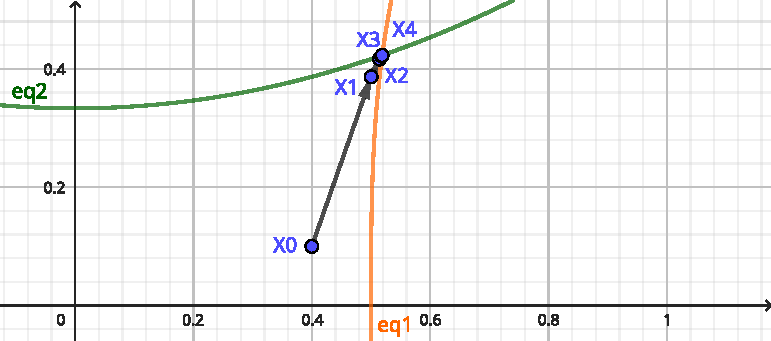
\includegraphics[width=0.6\textwidth]{img/sistema-não-linear-2x2-iteração-ponto-fixo-sequência.pdf}
\end{center}


\Exercise[title={2,5}] Utilize a forma de Newton do polinômio interpolador para estimar a temperatura máxima em uma cidade no mês de abril (\(4\)), considerando as temperaturas máximas nos 2 meses anteriores e nos 2 meses posteriores:
\medskip
\begin{center}
\begin{tabular}{cc}
\hline
Mês & Temperatura máxima (°C) \\
\hline
2 & 29 \\
3 & 31 \\
5 & 32 \\
6 & 28 \\
\hline
\end{tabular}
\end{center}
\medskip
{\color{blue} \textit{(Arredonde os valores obtidos com 3 casas decimais)}}

\Answer A partir dos pontos dados, obtém-se:
\[
\begin{array}{ccccc}
x_i
& y_i=f[x_i]
& f[x_i,x_{i+1}]
& f[x_i,x_{i+1},x_{i+2}]
& f[x_i,\ldots,x_{i+3}]\\
2 & \mathbf{29} \\
        & & \mathbf{2} \\
3 & 31 & & \mathbf{-0,5} \\
        & & 0,5 & & \mathbf{-0,25}. \\
5 & 32 & & -1,5 \\
        & & -4 \\
6 & 28
\end{array}
\]

Então:
\[
p(x) = 29 + 2\cdot(x-2) + (-0,5)\cdot(x-2)(x-3) + (-0,25)\cdot(x-2)(x-3)(x-5).
\]
Alternativamente, podemos reescrever o polinômio como
\[
p(x) = 29 + (x-2)\cdot\left[2 + (x-3)\cdot\left[-0,5 + (x-5) \cdot (-0,25)\right]\right].
\]
ou simplificá-lo para
\[
p(x) = -0,25 x^3 + 2 x^2 - 3,25 x + 29,5.
\]
Usando $p(x)$ para calcular o valor pedido, estima-se que a temperatura máxima em abril (em graus) seja dada por:
\[
p(x)
= 29 + 2\cdot\left[2 + 1\cdot\left[-0,5 + (-1) \cdot (-0,25)\right]\right]
= 32,5.
\]
Portanto, a temperatura máxima estimada para o mês de abril é de $\boxed{32,5^\circ}$.
\begin{center}
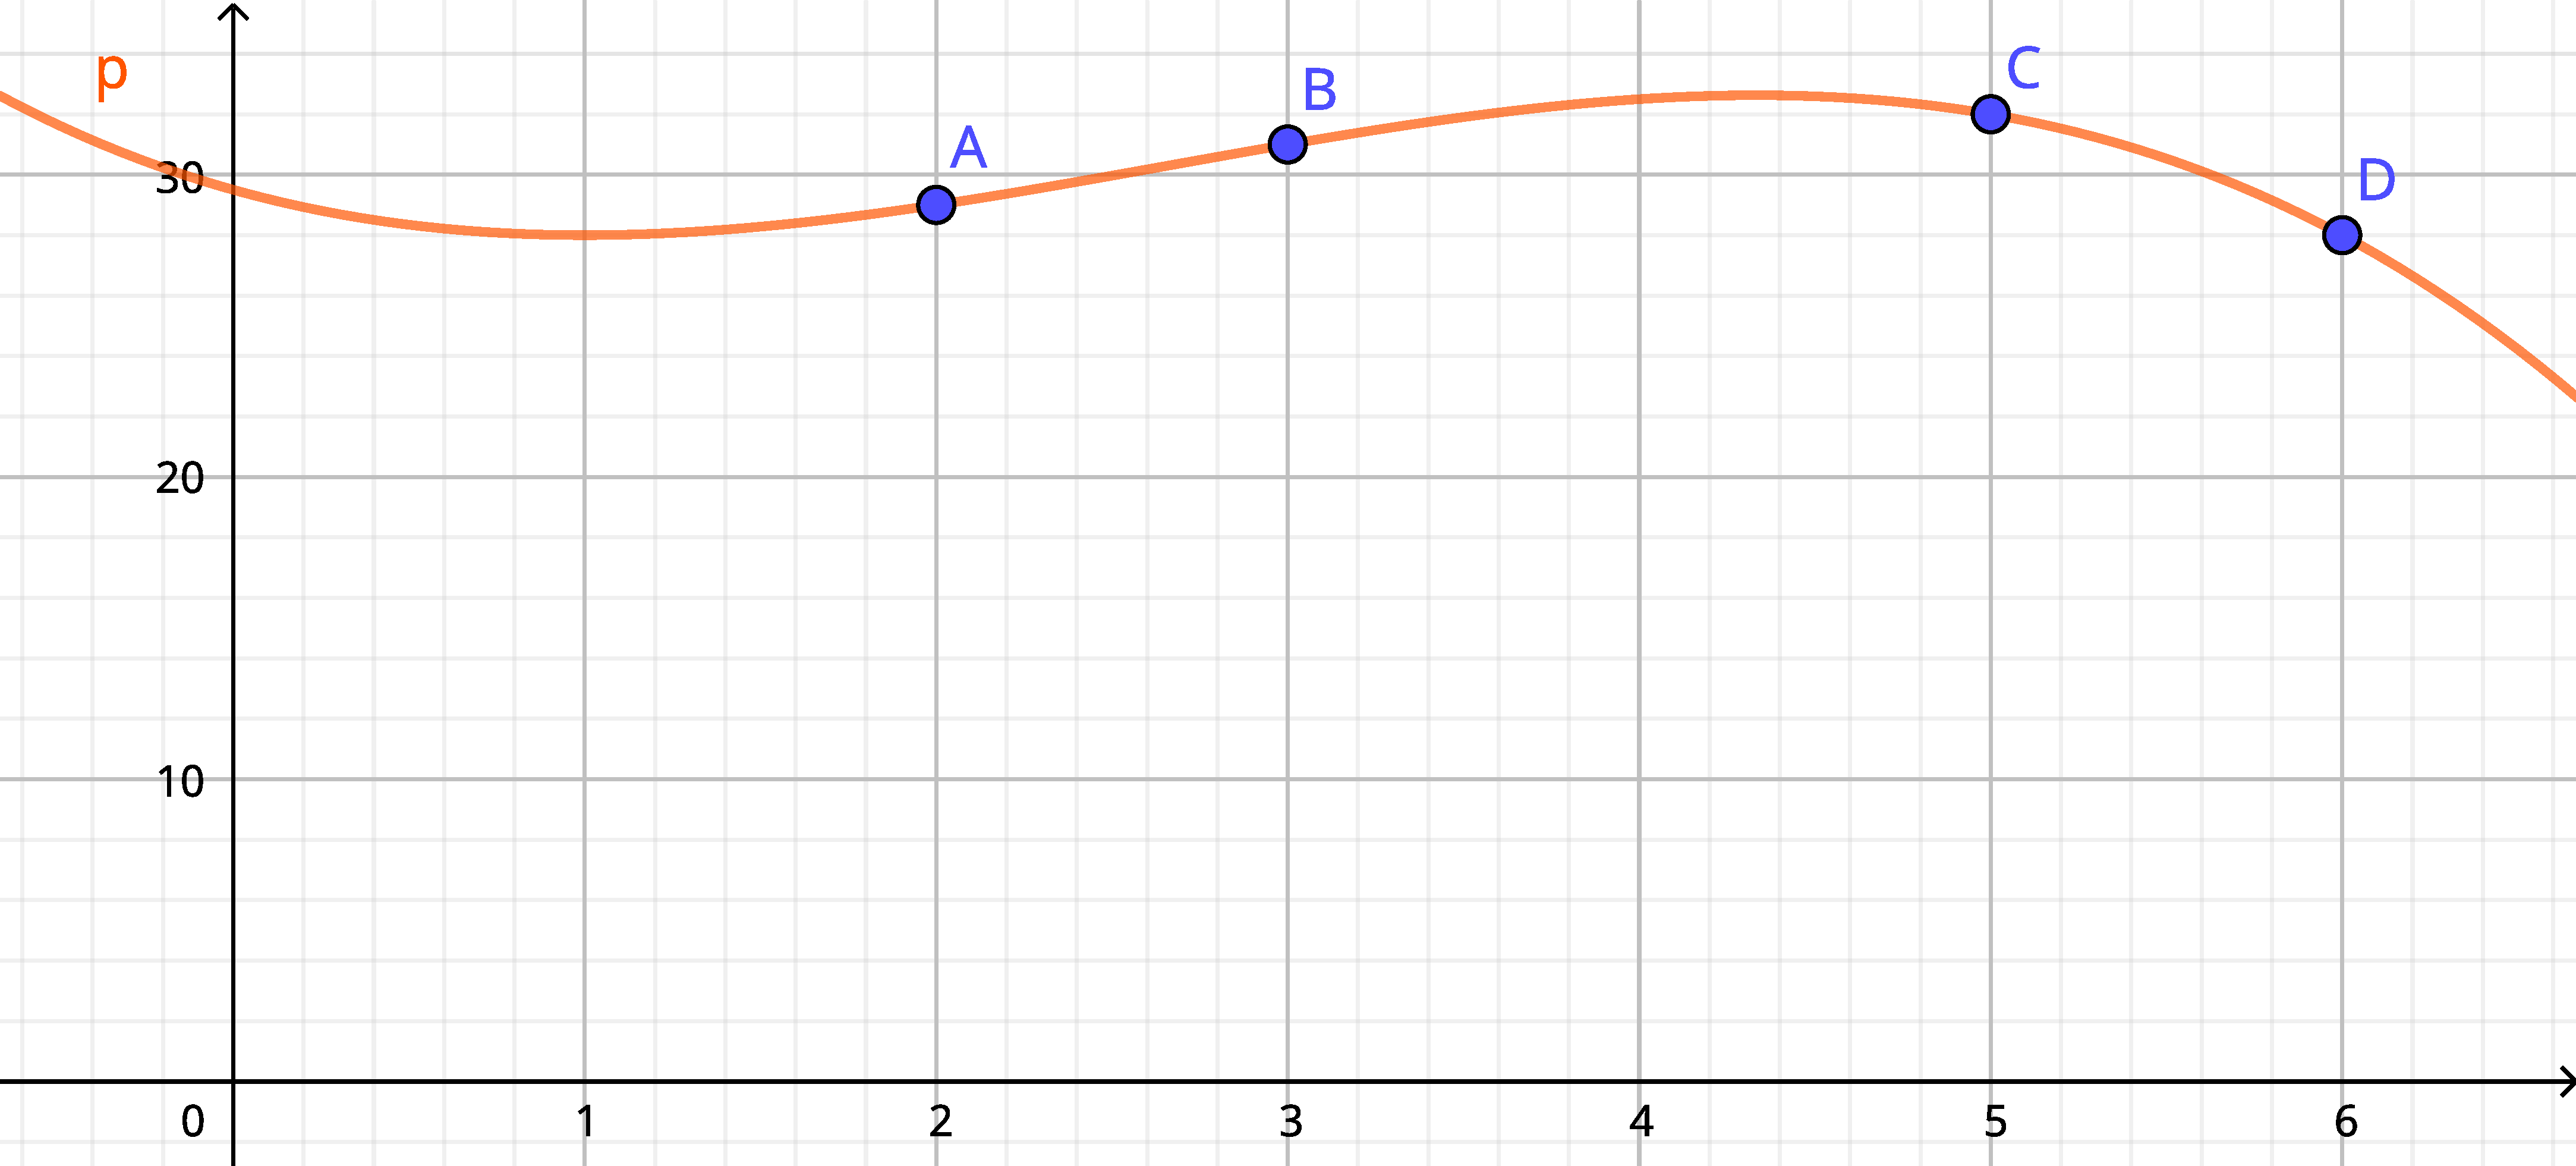
\includegraphics[width=0.6\textwidth]{img/interpolação-diferenças-divididas-newton-temperaturas.pdf}
\end{center}

\Exercise[title={2,5}] Sabendo que o spline cúbico natural \( s(x) \) que interpola os pontos \( (-1, 1) \), \( (1, 5) \) e \( (2, 1) \) satisfaz \( s'(-1) = 4 \), \( s'(1) = -2 \) e \( s'(2) = -5 \), escreva \( s(x) \) explicitamente.
\Answer Considerando os pontos dados, o spline tem a forma
\[
  s(x) =
  \begin{cases}
    a_0 + b_0(x + 1) + c_0(x + 1)^2 + d_0(x + 1)^3, & \text{se } -1 \leq x \leq 1,\\
    a_1 + b_1(x - 1) + c_1(x - 1)^2 + d_1(x - 1)^3, & \text{se } 1 \leq x \leq 2.
  \end{cases}
\]
Os valores de \( a_i \), \( b_i \), \( c_i \) e \( d_i \), para $i \in \{0, 1\}$ podem ser determinados de duas maneiras:

\textbf{Alternativa 1}: a partir das condições fornecidas, considere $y'_0 = s'(-1) = 4$, $y'_1 = s'(1) = -2$ e $y'_2 = s'(2) = -5$.

Para o intervalo \( -1 \leq x \leq 1 \), definindo $h_0 = x_1 - x_0 = 1 - (-1) = 2$, temos:
\[
\begin{cases}
  a_0 = y_0 = 1,\\
  b_0 = y'_0 = 4,\\
  c_0 = 3 \frac{y_1 - y_0}{h_0^2} - \frac{y'_1 + 2 y'_0}{h_0}
      = 3 \cdot \frac{5 - 1}{2^2} - \frac{-2 + 2 \cdot 4}{2}
      = 0,\\
  d_0 = -2 \frac{y_1 - y_0}{h_0^3} + \frac{y'_1 + y'_0}{h_0^2}
      = -2 \cdot \frac{5 - 1}{2^3} + \frac{-2 + 4}{2^2}
      = -\frac{1}{2}
      = -0,5.
\end{cases}
\]
e para o intervalo \( 1 \leq x \leq 2 \), definindo $h_1 = x_2 - x_1 = 2 - 1 = 1$, temos:
\[
\begin{cases}
  a_1 = y_1 = 5,\\
  b_1 = y'_1 = -2,\\
  c_1 = 3 \frac{y_2 - y_1}{h_1^2} - \frac{y'_2 + 2 y'_1}{h_1}
      = 3 \cdot \frac{1 - 5}{1^2} - \frac{-5 + 2 \cdot (-2)}{1}
      = -3,\\
  d_1 = -2 \frac{y_2 - y_1}{h_1^3} + \frac{y'_2 + y'_1}{h_1^2}
      = -2 \cdot \frac{1 - 5}{1^3} + \frac{-5 - 2}{1^2}
      = 1.
\end{cases}
\]

\textbf{Alternativa 2}: Primeiramente, usando os valores conhecidos de \(s\) e \(s'\) em \(x_0 = -1\), tem-se:
\[
  \begin{cases}
    s(-1) & = 1, \\
    s'(-1) & = 4
  \end{cases}
  \Rightarrow
  \begin{cases}
    a_0 + b_0\cdot 0 + c_0\cdot 0^2 + d_0\cdot 0^3 & = 1, \\
    b_0 + 2c_0\cdot 0 + 3d_0\cdot 0^2 & = 4
  \end{cases}
  \Rightarrow
  \begin{cases}
    a_0 & = 1, \\
    b_0 & = 4.
  \end{cases}
\]
Consequentemente, usando os valores conhecidos de \(s\) e \(s'\) em \(x_1 = 1\), tem-se:
\[
  \begin{cases}
    s(1) & = 5, \\
    s'(1) & = -2
  \end{cases}
  \Rightarrow
  \begin{cases}
    1 + 4\cdot 2 + c_0\cdot 2^2 + d_0\cdot 2^3 & = 5, \\
    4 + 2c_0\cdot 2 + 3d_0\cdot 2^2 & = -2
  \end{cases}
  \Rightarrow
  \begin{cases}
    4c_0 + 8d_0 & = -4, \\
    4c_0 + 12d_0 & = -6.
  \end{cases}
\]
Usando Cramer, conclui-se que \(c_0 = \frac{0}{16} = 0\) e \(d_0 = -\frac{8}{16} = -\frac{1}{2}\).

Na sequência, usando os valores conhecidos de \(s\) e \(s'\) em \(x_1 = 1\), resulta que
\[
  \begin{cases}
    s(1) & = 5, \\
    s'(1) & = -2
  \end{cases}
  \Rightarrow
  \begin{cases}
    a_1 + b_1\cdot 0 + c_1\cdot 0^2 + d_1\cdot 0^3 & = 5, \\
    b_1 + 2c_1\cdot 0 + 3d_1\cdot 0^2 & = -2
  \end{cases}
  \Rightarrow
  \begin{cases}
    a_1 & = 5, \\
    b_1 & = -2.
  \end{cases}
\]
Consequentemente, usando os valores conhecidos de \(s\) e \(s'\) em \(x_2 = 2\), tem-se:

\[
  \begin{cases}
    s(2) & = 1, \\
    s'(2) & = -5
  \end{cases}
  \Rightarrow
  \begin{cases}
    5 - 2\cdot 1 + c_1\cdot 1^2 + d_1\cdot 1^3 & = 1, \\
    -2 + 2c_1 + 3d_1 & = -5
  \end{cases}
  \Rightarrow
  \begin{cases}
    c_1 + d_1 & = -2, \\
    2c_1 + 3d_1 & = -3.
  \end{cases}
\]
Por Cramer, obtém-se \(c_1 = \frac{-3}{1} = -3\) e \(d_1 = \frac{1}{1} = 1\).

Portanto, substituindo os valores obtidos, o spline cúbico \( s(x) \) é dado por
\[
\boxed{
  s(x) =
  \begin{cases}
    1 + 4(x + 1) + 0(x + 1)^2 - 0.5(x + 1)^3, & \text{se } -1 \leq x \leq 1,\\
    5 - 2(x - 1) - 3(x - 1)^2 + 1(x - 1)^3, & \text{se } 1 \leq x \leq 2.
  \end{cases}
}
\]

\textit{Observação}: Para fins de validação, note que \( s(-1) = 1 \), \( s(1) = 5 \) e \( s(2) = 1 \), como esperado. Graficamente, $s(x)$ tem a seguinte representação:

\begin{center}
  \includegraphics[width=8.0cm]{img/spline-de-ordem-3-natural-3-nós-coeficientes-racionais.pdf}
\end{center}


\Exercise[title={2,5}] Calcule o resíduo quadrático da função do tipo
\[
f(x) = a_1 x^2 + a_2 \cos(\pi x)
\]
que melhor se ajusta, no sentido dos mínimos quadrados, aos pontos do conjunto
\[
D = \{(-1, -1), (0, 1), (1, -2), (2, -1)\}.
\]

\Answer
Sejam $P_1 = (-1, -1)$, $P_2 = (0, 1)$, $P_3 = (1, -2)$, $P_4 = (2, -1)$ e considere $g_1(x) = x^2$ e $g_2(x) = \cos(\pi x)$. Para encontrar uma função da forma $q(x) = a_1 g_1(x) + a_2 g_2(x)$ que melhor se ajusta aos pontos $P_i = (x_i, y_i)$, para $1 \leq i \leq 4$, basta resolver o sistema $A^T A X = A^T B$, em que
\[
A =
\begin{bmatrix}
g_1(x_1) & g_2(x_1) \\
g_1(x_2) & g_2(x_2) \\
g_1(x_3) & g_2(x_3) \\
g_1(x_4) & g_2(x_4)
\end{bmatrix}
=
\begin{bmatrix}
(-1)^2 & \cos(-\pi) \\
0^2 & \cos(0) \\
1^2 & \cos(\pi) \\
2^2 & \cos(2\pi)
\end{bmatrix}
=
\begin{bmatrix}
1 & -1 \\
0 &  1 \\
1 & -1 \\
4 &  1
\end{bmatrix},
\quad
X =
\begin{bmatrix}
a_1\\a_2
\end{bmatrix},
\quad
B =
\begin{bmatrix}
-1 \\
1 \\
-2 \\
-1
\end{bmatrix},
\]

Considerando os dados fornecidos, tem-se:
\[
A^T A
=
\begin{bmatrix}
 1 & 0 &  1 & 4 \\
-1 & 1 & -1 & 1
\end{bmatrix}
\cdot
\begin{bmatrix}
1 & -1 \\
0 &  1 \\
1 & -1 \\
4 &  1
\end{bmatrix}
=
\begin{bmatrix}
18 & 2 \\
2 & 4
\end{bmatrix},
\]
e
\[
A^T B
=
\begin{bmatrix}
1 & 0 &  1 & 4 \\
-1 & 1 & -1 & 1
\end{bmatrix}
\begin{bmatrix}
-1 \\
1 \\
-2 \\
-1
\end{bmatrix}
=
\begin{bmatrix}
-7 \\ 3
\end{bmatrix}.
\]

Então,
\[
A^T A X = A^T B
\Leftrightarrow
\begin{bmatrix}
18 & 2 \\
2 & 4
\end{bmatrix}
\cdot
\begin{bmatrix}
a_1\\
a_2
\end{bmatrix}
=
\begin{bmatrix}
-7 \\ 3
\end{bmatrix}
\Leftrightarrow
\begin{bmatrix}
a_1\\
a_2
\end{bmatrix}
=
\begin{bmatrix}
-1/2\\
1
\end{bmatrix}.
\]

Portanto, a função é $q(x) = -\frac{1}{2}x^2 + \cos(\pi x)$. O resíduo quadrático é dado por
\begin{align*}
R
&= \sum_{i=1}^{4} (q(x_i) - y_i)^2 \\
&= \left(-\frac{1}{2}(-1)^2 + \cos(-\pi) + 1\right)^2 + \left(-\frac{1}{2}(0)^2 + \cos(0) - 1\right)^2 \\
&\quad + \left(-\frac{1}{2}(1)^2 + \cos(\pi) + 2\right)^2 + \left(-\frac{1}{2}(2)^2 + \cos(2\pi) + 1\right)^2 \\
&= \left(-\frac{1}{2} - 1 + 1\right)^2 + (1 - 1)^2 + \left(-\frac{1}{2} - 1 + 2\right)^2 + \left(-2 + 1 + 1\right)^2 \\
&= \left(-\frac{1}{2}\right)^2 + 0^2 + \left(\frac{1}{2}\right)^2 + 0^2 = \frac{1}{4} + \frac{1}{4} = \boxed{\frac{1}{2}}.
\end{align*}
O gráfico de $f(x)$ é o seguinte:
\begin{center}
  \includegraphics[width=8.0cm]{img/ajuste-mínimos-quadrados-4-pontos-matrizes-trig.pdf}
\end{center}
\end{ExerciseList}

\vfill
\begin{center}
BOA PROVA!
\end{center}

\newpage
\restoregeometry
\section*{Respostas}
\shipoutAnswer
\end{document}
